\documentclass{article}
\title{Ch. 5 CW Pt. 1}
\usepackage{graphicx, amsmath}
\graphicspath{ {./images/} }

\author{Principles of Microeconomics}
\date{\today}

\begin{document}

\maketitle

\begin{enumerate}

\item (c) -- If the demand curve is inelastic, an increase in supply will decrease price proportionately more than it will increase quantity. As a result, revenue will go down.

\begin{center}
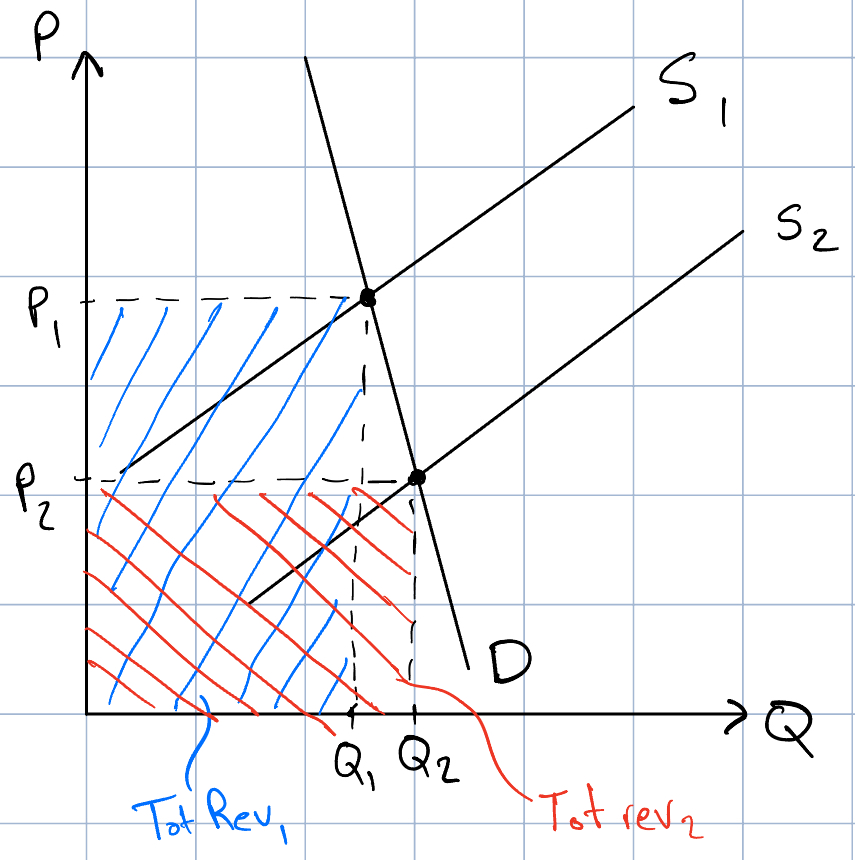
\includegraphics[width = 0.5\textwidth]{problem1}
\end{center}

\item (b) -- For total expenditure (a.k.a. revenue) to increase when price goes down, quantity must increase proportionately more than price decreases. That means the numerator of the price elasticity of demand equation must be bigger than the denominator, so the price elasticity of demand must be zero. Additionally, for quantity to go up when incomes go up, smartphones must be a normal good. That means the income elasticity of demand must be greater than 0. 

\item

	\begin{enumerate}
	
	\item The hurricane decreases the supply of coffee beans, so supply shifts left. As a result, price increases.
	
	\begin{center}
	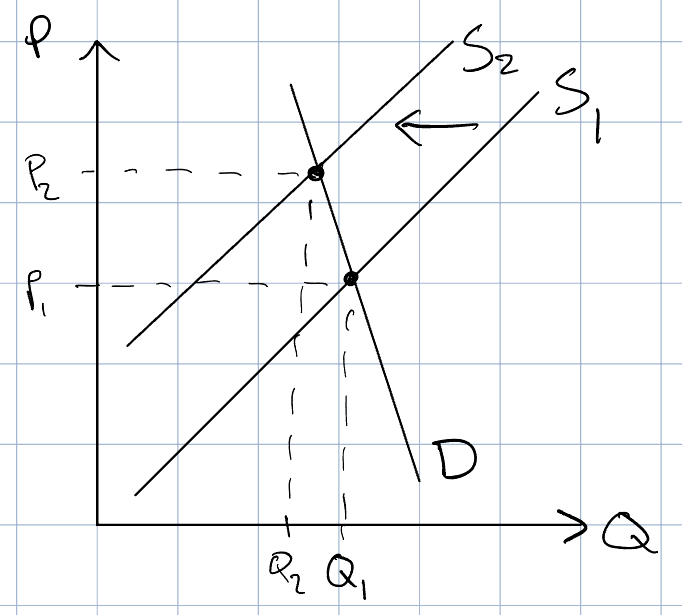
\includegraphics[width = 0.5\textwidth]{problem3a}
	\end{center}
	
	\item Because the price of coffee beans, an input, increased, the supply of cups shifts left. As a result price increases, and quantity decreases. Since demand is inelastic, the increase in price is proportionately larger than the decrease in quantity. That means total expenditure increases.
	
	\begin{center}
	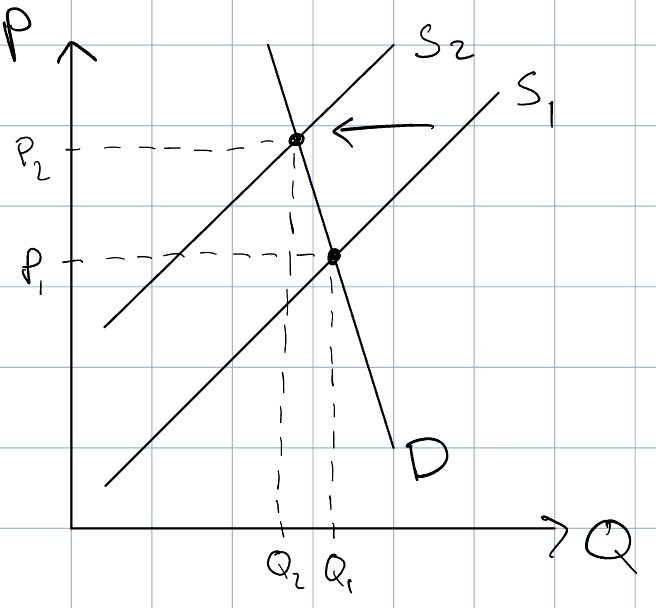
\includegraphics[width = 0.5\textwidth]{problem3b}
	\end{center}
	
	\newpage
	
	\item The price of a complement went up, so demand for donuts decreases. Therefore, quantity and price both decrease which means total expenditure decreases as well.
	
	\begin{center}
	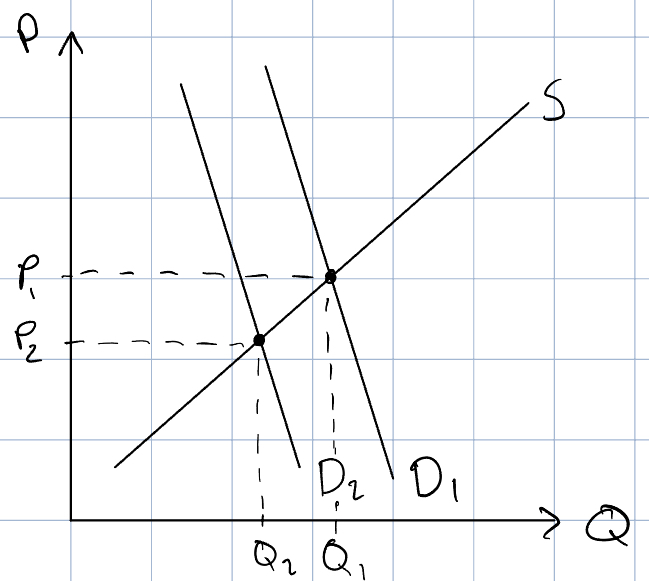
\includegraphics[width = 0.5\textwidth]{problem3c}
	\end{center}
	
	\end{enumerate}

\newpage

\item \phantom{x} \\

\begin{center}
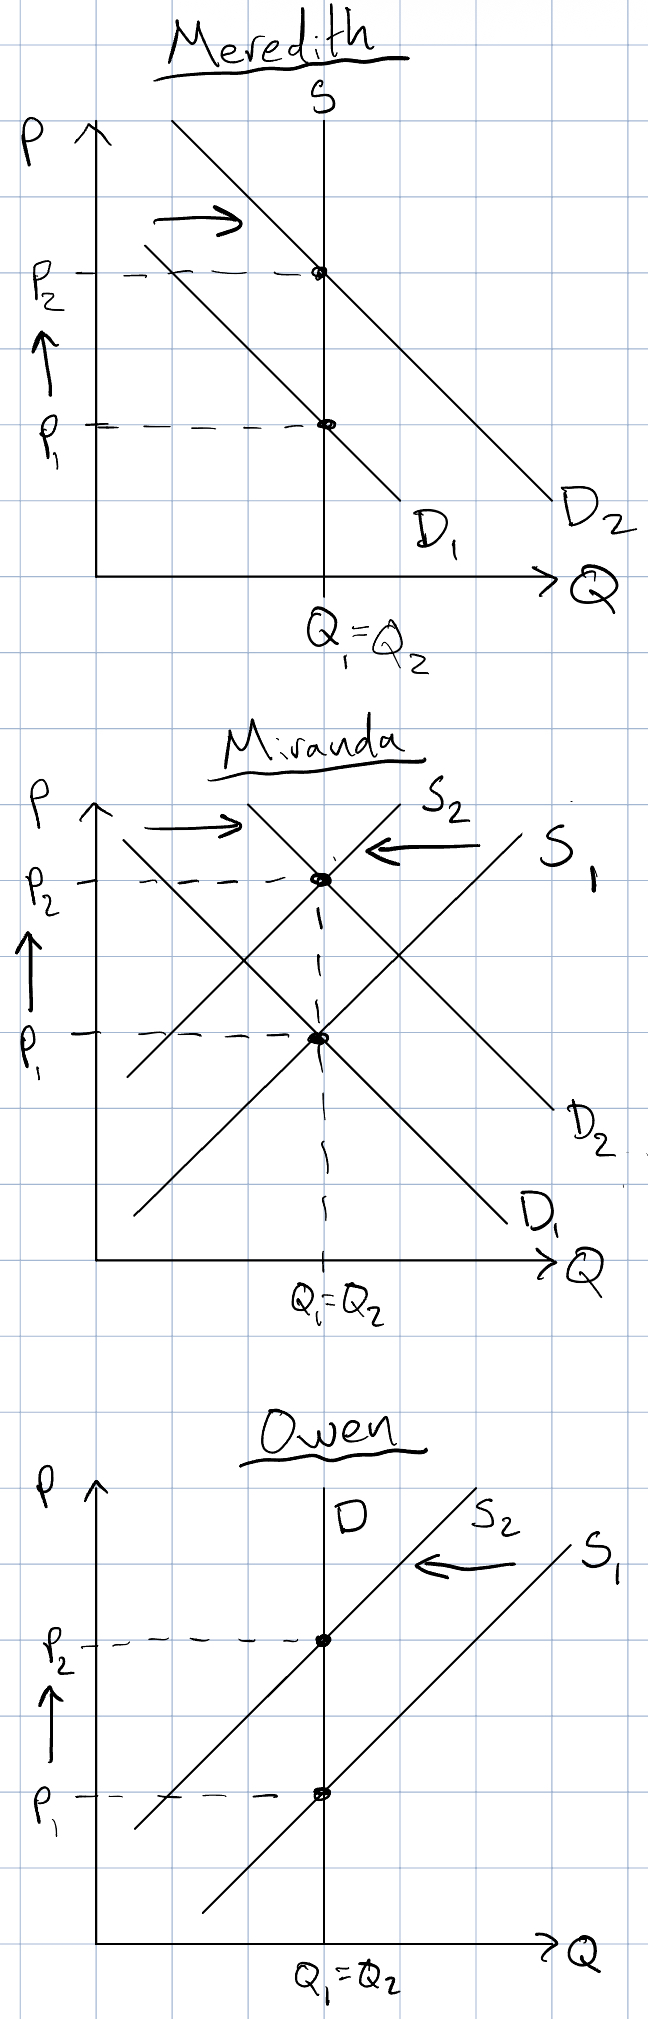
\includegraphics[width = 0.45\textwidth]{problem4}
\end{center}

\item It depends on the price elasticity of demand for museum admission. If demand is elastic, the museum should decrease the price of admission because the quantity of admits will increase proportionately more than price will decrease. If demand is inelastic, the museum should increase the price of admission because the quantity of admits will decrease proportionately less than price will increase. I imagine demand for museum admission is elastic because it's a highly substitutable activity.

\item A drought around the world will shift supply left. If we assume that demand for grains is inelastic because grains are a staple food, then price will increase proportionately more than quantity will decrease (see the figure for \#1). That means total revenue will increase.

A drought only in Kansas might have a minimal effect on the world supply of grain because Kansas might make up a minimal share of the world grain market. That means supply will shift left and the price of grains will increase minimally if at all. Therefore, Kansas farmers will sell a significantly smaller quantity of grains, but they'll receive a minimally higher price. As a result, Kansas farmers might make less revenue due to the drought.

\end{enumerate}

\end{document}